\documentclass[12pt]{article}
 \usepackage[margin=1in]{geometry} 
\usepackage{amsmath,amsthm,amssymb,amsfonts}
\usepackage{graphics} 
\usepackage[dvipdfmx]{graphicx}

\newcommand{\N}{\mathbb{N}}
\newcommand{\Z}{\mathbb{Z}}
 
\newenvironment{problem}[2][Problem]{\begin{trivlist}
\item[\hskip \labelsep {\bfseries #1}\hskip \labelsep {\bfseries #2.}]}{\end{trivlist}}
%If you want to title your bold things something different just make another thing exactly like this but replace "problem" with the name of the thing you want, like theorem or lemma or whatever
 
\begin{document}
 
%\renewcommand{\qedsymbol}{\filledbox}
%Good resources for looking up how to do stuff:
%Binary operators: http://www.access2science.com/latex/Binary.html
%General help: http://en.wikibooks.org/wiki/LaTeX/Mathematics
%Or just google stuff
 
\title{HW 1}
\author{Motoaki Takahashi}
\maketitle
\section{Question 1}

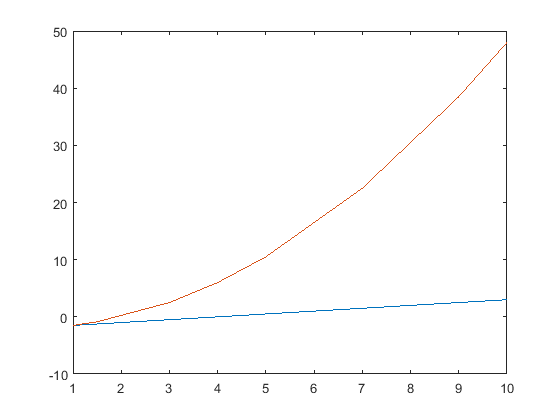
\includegraphics{q1.png}\par
$Y1$ and $Y2$ are shown above, where the blue line is $Y1$ and the red curve is $Y2$.

\section{Question 2}
The $200\times1$ vector that contains evenly-spaced numbers between $[-10, 20]$ is 
$$
( -10.0000, -9.8492, -9.6985, \cdots, 19.6985, 19.8492, 20.0000).
$$
The full expression is given in the diary file, hw1.out.

\section{Question 3}
$$
C=\left[
\begin{array}{c}
    29\\
   133\\
43
\end{array}
\right],
$$

$$
D=\left[
\begin{array}{c}
   -3.2505\\
    0.3961\\
0.8037
\end{array}
\right],
$$

$$
E=205,
$$

$$
F=\left[
\begin{array}{cc}
     2, &    4\\
3, & 12
\end{array}
\right],
$$

$$
x=\left[
\begin{array}{c}
   -0.1622\\
    1.2432\\
-1.1081
\end{array}
\right].
$$

\section{Question 4}
$B$ is the Kronecker product of the $5\times 5$ identity matrix and $A$ in question 3. This yields
$$
B=\left[
\begin{array}{ccccccccccccccc}
     2   &  4 &    6 &    0 &    0 &    0  &   0 &    0 &    0 &    0 &    0 &    0 &    0 &    0 &    0\\
     1  &   7 &    5 &    0 &    0 &    0 &    0 &    0 &    0 &    0 &    0 &    0 &    0 &    0 &    0\\
     3 &   12&     4   &  0   &  0  &   0  &   0  &   0 &    0 &    0 &    0 &    0 &    0  &   0  &   0\\
     0 &    0  &   0   &  2   &  4 &    6&     0 &    0    & 0 &    0  &   0   &  0     &0  &   0 &    0\\
     0   &  0   &  0  &   1 &    7   &  5  &   0   &  0 &    0   &  0&     0  &   0 &    0 &    0&     0\\
     0  &   0 &    0  &   3   & 12    & 4   &  0 &    0 &    0 &    0  &   0  &   0    & 0  &   0  &   0\\
     0  &   0 &    0&     0&     0&     0&     2&     4&     6&     0&     0&     0&     0&     0&     0\\
     0   &  0  &   0 &    0 &    0&     0&     1&     7&     5&     0&     0 &    0&     0&     0&     0\\
     0    & 0   &  0  &   0  &   0&     0&     3&    12&     4&     0&     0&     0&     0&     0&     0\\
     0   &  0  &   0   &  0   &  0 &    0&     0&     0 &    0 &    2&     4&     6 &    0 &    0 &    0\\
     0    & 0   &  0    & 0&     0  &   0 &    0 &    0 &    0&     1 &    7 &    5 &    0 &    0  &   0\\
     0  &   0   &  0&     0 &    0   &  0  &   0  &   0 &    0 &    3  &  12 &    4&     0&     0  &   0\\
     0   &  0   &  0 &    0  &   0   &  0   &  0   &  0 &    0 &    0   &  0   &  0 &    2 &    4  &   6\\
     0    & 0   &  0 &    0   &  0   &  0     &0    & 0 &    0 &    0    & 0    & 0 &    1 &    7  &   5\\
    0 &0 &0 &0& 0& 0& 0& 0& 0& 0& 0& 0& 3& 12& 4
\end{array}
\right].
$$

\section{Question 5}
I happen to have the following result.
$$
A=\left[
\begin{array}{rrr}
    6.9984&   -0.6918&   10.6202\\
   12.4498&    5.8021 &  17.1835\\
   13.6968 &  16.7730&    0.1955\\
   18.5594  &  4.6392  &  9.0115\\
9.0294& 14.8048& 3.9608
\end{array}
\right],
$$

$$
B=\left[
\begin{array}{rrr}
   0&   0&   1\\
   1 &  0&   1\\
   1 &  1&   0\\
   1 &  0 &  0\\
   0 &1& 0
\end{array}
\right]
$$.

\section{Question 6}
I constructed the matrix $X$ that contains 1's in the 1st column, and the export dummy, the R\&D dummy and capital stock in the 2nd, 3rd and 4th columns respectively. The vector $y$ is the column vector that contains the productivity index for each observation. Then the OLS estimate is
$$
\hat{\beta}=(X'X)^{-1}X'y=\left[
\begin{array}{r}
    0.0817\\
    0.1201\\
    0.1399\\
0.0295
\end{array}
\right].
$$
Let the residual vector $e$ be $e=y-X\hat{\beta}$. Let $p$ be the number of the explanatory variables, that is 4. Then the standard errors are the square roots of the diagonal elements of
$$
\hat{V}[\hat{\beta}|\ X]=\frac{e'e}{n-p}(X'X)^{-1}.
$$
The standard errors are
$$
\left[
\begin{array}{r}
    0.0167\\
    0.0063\\
    0.0085\\
0.0018
\end{array}
\right].
$$
\section{Code}
The following is the matlab code for HW1, copied from HW1.m.
\begin{small}
\begin{verbatim}
% Motoaki Takahashi
% HW1 for Econ 512 Empirical Methods
clear

diary hw1.out


%% Question 1
disp('Question 1')

X=[1, 1.5, 3, 4, 5, 7, 9, 10];
Y1=-2+0.5*X
Y2=-2+0.5*(X.^2)
Y=[Y1; Y2]
plot(X, Y)

%% Question 2
disp('Question 2')

X=linspace(-10, 20, 200)

%% Question 3
disp('Question 3')

A=[2, 4, 6;
   1, 7, 5;
   3, 12, 4];

b=[-2; 3; 10];

C=A.'*b
D=inv(A.'*A)*b
E=sum(b.'*A)
F=A([1,3],[1,2])

% solve the system of linear equations for the vector x
x=inv(A)*b

%% Question 4
disp('Question 4')

B=kron(eye(5,5), A)

%% Question 5
disp('Question 5')

% 5X3 matrix whose elements are random draws from N(10, 5^2)
A=normrnd(10, 5, [5,3])
% B has an element 1 if the correspondent in A is bigger than or equal to 10
B=A>=10

%% Question 6
disp('Question 6')

% read the csv file
data='datahw1.csv';
data=csvread(data);
% X is a matrix of explanatory variables
X=data(1:size(data,1),[3,4,6]);
X=[ones(size(data,1),1), X];

% y is a vector of a explained variable
y=data(1:size(data,1), 5);

% OLS estimate
disp('OLS estimate')
b=inv(X.'*X)*(X.'*y)

% residual
e= y -X*b;
% the estimate for the variance of beta-hat (here b)
Var_hat=((e'*e)/(size(data,1)-4))*inv(X'*X);
disp('Standard Errors')
se=diag(Var_hat.^(1/2))

diary off
\end{verbatim}
\end{small}

\section{Output}
The following is the output on matlab (except for the graph), which is copied from hw1.out.

\fontsize{7.3pt}{3pt}\selectfont
\begin{verbatim}
Question 1

Y1 =

   -1.5000   -1.2500   -0.5000         0    0.5000    1.5000    2.5000    3.0000


Y2 =

   -1.5000   -0.8750    2.5000    6.0000   10.5000   22.5000   38.5000   48.0000


Y =

   -1.5000   -1.2500   -0.5000         0    0.5000    1.5000    2.5000    3.0000
   -1.5000   -0.8750    2.5000    6.0000   10.5000   22.5000   38.5000   48.0000


Question 2

X =

  Columns 1 through 14

  -10.0000   -9.8492   -9.6985   -9.5477   -9.3970   -9.2462   -9.0955   -8.9447   -8.7940   -8.6432   -8.4925   -8.3417   -8.1910   -8.0402

  Columns 15 through 28

   -7.8894   -7.7387   -7.5879   -7.4372   -7.2864   -7.1357   -6.9849   -6.8342   -6.6834   -6.5327   -6.3819   -6.2312   -6.0804   -5.9296

  Columns 29 through 42

   -5.7789   -5.6281   -5.4774   -5.3266   -5.1759   -5.0251   -4.8744   -4.7236   -4.5729   -4.4221   -4.2714   -4.1206   -3.9698   -3.8191

  Columns 43 through 56

   -3.6683   -3.5176   -3.3668   -3.2161   -3.0653   -2.9146   -2.7638   -2.6131   -2.4623   -2.3116   -2.1608   -2.0101   -1.8593   -1.7085

  Columns 57 through 70

   -1.5578   -1.4070   -1.2563   -1.1055   -0.9548   -0.8040   -0.6533   -0.5025   -0.3518   -0.2010   -0.0503    0.1005    0.2513    0.4020

  Columns 71 through 84

    0.5528    0.7035    0.8543    1.0050    1.1558    1.3065    1.4573    1.6080    1.7588    1.9095    2.0603    2.2111    2.3618    2.5126

  Columns 85 through 98

    2.6633    2.8141    2.9648    3.1156    3.2663    3.4171    3.5678    3.7186    3.8693    4.0201    4.1709    4.3216    4.4724    4.6231

  Columns 99 through 112

    4.7739    4.9246    5.0754    5.2261    5.3769    5.5276    5.6784    5.8291    5.9799    6.1307    6.2814    6.4322    6.5829    6.7337

  Columns 113 through 126

    6.8844    7.0352    7.1859    7.3367    7.4874    7.6382    7.7889    7.9397    8.0905    8.2412    8.3920    8.5427    8.6935    8.8442

  Columns 127 through 140

    8.9950    9.1457    9.2965    9.4472    9.5980    9.7487    9.8995   10.0503   10.2010   10.3518   10.5025   10.6533   10.8040   10.9548

  Columns 141 through 154

   11.1055   11.2563   11.4070   11.5578   11.7085   11.8593   12.0101   12.1608   12.3116   12.4623   12.6131   12.7638   12.9146   13.0653

  Columns 155 through 168

   13.2161   13.3668   13.5176   13.6683   13.8191   13.9698   14.1206   14.2714   14.4221   14.5729   14.7236   14.8744   15.0251   15.1759

  Columns 169 through 182

   15.3266   15.4774   15.6281   15.7789   15.9296   16.0804   16.2312   16.3819   16.5327   16.6834   16.8342   16.9849   17.1357   17.2864

  Columns 183 through 196

   17.4372   17.5879   17.7387   17.8894   18.0402   18.1910   18.3417   18.4925   18.6432   18.7940   18.9447   19.0955   19.2462   19.3970

  Columns 197 through 200

   19.5477   19.6985   19.8492   20.0000


Question 3

C =

    29
   133
    43


D =

   -3.2505
    0.3961
    0.8037


E =

   205


F =

     2     4
     3    12


x =

   -0.1622
    1.2432
   -1.1081


Question 4

B =

     2     4     6     0     0     0     0     0     0     0     0     0     0     0     0
     1     7     5     0     0     0     0     0     0     0     0     0     0     0     0
     3    12     4     0     0     0     0     0     0     0     0     0     0     0     0
     0     0     0     2     4     6     0     0     0     0     0     0     0     0     0
     0     0     0     1     7     5     0     0     0     0     0     0     0     0     0
     0     0     0     3    12     4     0     0     0     0     0     0     0     0     0
     0     0     0     0     0     0     2     4     6     0     0     0     0     0     0
     0     0     0     0     0     0     1     7     5     0     0     0     0     0     0
     0     0     0     0     0     0     3    12     4     0     0     0     0     0     0
     0     0     0     0     0     0     0     0     0     2     4     6     0     0     0
     0     0     0     0     0     0     0     0     0     1     7     5     0     0     0
     0     0     0     0     0     0     0     0     0     3    12     4     0     0     0
     0     0     0     0     0     0     0     0     0     0     0     0     2     4     6
     0     0     0     0     0     0     0     0     0     0     0     0     1     7     5
     0     0     0     0     0     0     0     0     0     0     0     0     3    12     4


Question 5

A =

    6.9984   -0.6918   10.6202
   12.4498    5.8021   17.1835
   13.6968   16.7730    0.1955
   18.5594    4.6392    9.0115
    9.0294   14.8048    3.9608


B =

   0   0   1
   1   0   1
   1   1   0
   1   0   0
   0   1   0


Question 6
OLS estimate

b =

    0.0817
    0.1201
    0.1399
    0.0295

Standard Errors

se =

    0.0167
    0.0063
    0.0085
    0.0018

\end{verbatim}


\end{document}

